
% ibs.tex

\documentclass[10pt,a4paper,titlepage]{article}
\usepackage[czech]{babel}
\usepackage[utf8]{inputenc}
\usepackage[margin=100pt]{geometry}
    
\usepackage{graphicx}   % Import pictures
\usepackage{multicol}
\usepackage{caption}
\usepackage{subcaption}
%\usepackage{csquotes}

\usepackage[backend=biber, sorting=none]{biblatex}
\addbibresource{ibs.bib}
    
\begin{document}
  \pagenumbering{gobble}

  \begin{center}
    \section*{Klasifikace situace na základě dat z PIR senzorů}
    Martin Beneš
  \end{center}

  \subsection*{Fyzikální podstata}
  PIR ({\it passive infrared}) senzor je elektrické zařízení, které snímá elektromagnetické záření
  o~vlnových délkách $\lambda\in<700~nm;2.5~mm>$, neboli frekvencích $f\in<120~MHz;430~THz>$.
  Takové záření je vysíláno každým objektem, jehož teplota je vyšší než absolutní nula, tedy
  $T_{obj}>-273.15~K$, při~které jsou entropie (náhodný pohyb částic) i entalpie (energie, uložena
  v termodynamickém systému) rovny nule. A právě náhodný pohyb nabitých částic (elektronů, protonů),
  ze~kterých se objekty skládají, zapřičiňuje vysílání energie ve~formě fotonů, též elektromagnetické
  záření.

  Elektromagnetická záření dělíme podle~jejich využití do~několika kategorií podle~vlnové délky $\lambda$,
  popř.~frekvence $f$. Tyto dvě charakteristiky jsou vzhledem ke~konstantní rychlosti šíření záření
  vzájemně převoditelné vztahem $f=\frac{c}{\lambda}$, kde~$c=3\cdot10^{8}~m\cdot s^{-1}$ je rychlost světla. 

  \begin{figure}[h!]
    \begin{center}
      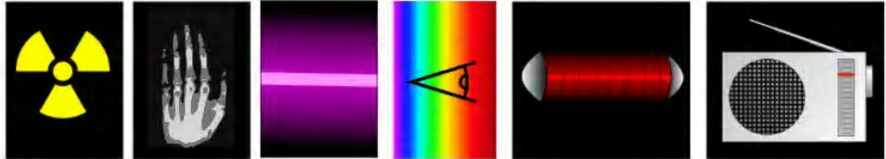
\includegraphics[width=0.5\textwidth]{spectrum.png}
      \caption[title=Obrazek]{Elektromagnetické spektrum\label{fig:spectrum} \cite{IZGcolors}}
    \end{center}    
  \end{figure}

  S~rostoucí $\lambda$ jsou to gamma záření, rentgen ({\it X-rays}), ultrafialové záření({\it UV}),
  viditelné světlo, infračervené záření ({\it IR}) a rádiové vlny. Obrázek \ref{fig:spectrum} ukazuje
  toto rozdělení. Někdy se také určuje pásmo mikrovln, nacházející se mezi~infračerveným a rádiovým.

  Infračervené záření se tedy vyskytuje běžně kolem nás a naše tělo jej vnímá jako teplotu. Energie
  takového záření (tzv. zářivá energie) se spočítá jako $W_e=h\cdot f$, kde $f$ je kmitočet záření
  a $h=6.63\cdot10^{-34}~J\cdot s $ je Planckova konstanta. \cite{WikipediaInfrared}

  \subsection*{Infračervené detektory}
  \paragraph*{Inspirace přírodou}
  Některé organismy jsou schopny vnímat infračervené záření a tím zvyšovat svoji šanci na přežití.
  Jedním z nich jsou někteří hadi (krajty, chřestýši, hroznýši...), kteří mají v obličeji velmi citlivé
  termoreceptory, které jim pomáhají v lovu teplokrevných živočichů. Díky jejich směrové citlivosti
  a toho, že jejich více, mohou přesně odhadovat směr a vzdálenost, kde se nachází kořist. \cite{SnakeInfrared}
  Živočichové, kteří se živí krví, např. upír obecný nebo jihoamerická ploštice Triatoma infestans,
  používají termoreceptory, aby poznali místo, kde je céva a kam tedy kousnout.

  \paragraph{Konstrukce}
  Při snímání je možné využít hned několik látek, které reagují na teplotu, a to tak, že je možné
  toto chování co nejpřesněji snímat elektrickým obvodem a vyhodnocovat počítačem. Podle
  charakteru jejich chování se detektory, které toho využívají, dělí na jednotlivé typy.
  {\it Bolometry} využívají změnu elektrického odporu vlivem ohřevu odporového elementu
  absorbovaným vstupním zářením. {\it Termoelektrické detektory} snímají změnu termoelektrického
  napětí dvojice vodičů vlivem rozdílu teplot mezi meřícím (ozářeným) a srovnávacím (zatemněným)
  spojem. {\it Pyroelektrické detektory} jsou založeny na elektrostatické polarizaci, měnící se při
  změně teplot. \cite{DetectorsBook}

  Stejně tak, jako chřestýši jsou schopni určovat přesnou pozici kořisti, je pro reálné využití detektoru
  při snímání a rozpoznávání třeba dosáhnout směrové citlivosti. Proto se používá podobná technika jako
  u fotoaparátů, jednotlivé jednoduché snímače se umístí do matice a data, které tyto snímače produkují,
  jsou poté řetězcem výpočetních jednotek zpracovávány do požadovaného výstupního formátu.
  
  \subsection*{Klasifikace}
  Klasifikace je druh problému, kteří řeší, do které z tříd (kategorií) dat patří nové pozorování.
  Pozorování se reprezentuje pomocí příznaků ({\it features}), které jsou
  diskriminativní, tedy rozlišují mezi třídami, invariantní vůči případným transformací (translaci,
  rotaci, změně měřítka atd.) a dekorelované. 

  Po získání takovýchto příznaků je zpracovává klasifikační systém, který přiřazuje n-tici příznaků
  jako celek k nějaké třídě. Nejčastěji používá fuzzy logiku, pomocí které vyjádří neurčitost přiřazení,
  v takovém případě tvrdé rozhodnutí (pokud je nutné) dělá postprocessor, který zvažuje také ceny
  rozhodnutí pro jednotlivé třídy. Tato konfigurace stanovuje tzv. DET křivku, udávající poměr mezi
  pravděpodobností nerozpoznaného výskytu a "falešným poplachem". \cite{IKRclassification}



  %\cite{BodilySenses}

  
  % references
  \printbibliography

\end{document}